\glspl{uav}, commonly referred to as drones, have become essential tools across a wide range of applications, including surveying, inspection, and research. Their ability to operate in confined or inaccessible environments makes them particularly valuable for close-range observation and monitoring tasks. Unlike outdoor drones that rely on satellite-based positioning systems such as GPS, indoor platforms must depend entirely on onboard sensing, control algorithms, and communication systems to maintain stability and navigate safely. Operating in enclosed environments presents additional challenges, including limited spatial awareness, airflow disturbances, and increased safety risks due to proximity to structures and personnel. Consequently, the design of an indoor \gls{uav} demands careful consideration of system architecture, control robustness, and physical safety features. 

\begin{figure}[H]
    \centering
    \captionsetup{justification=centering, margin=1cm}
    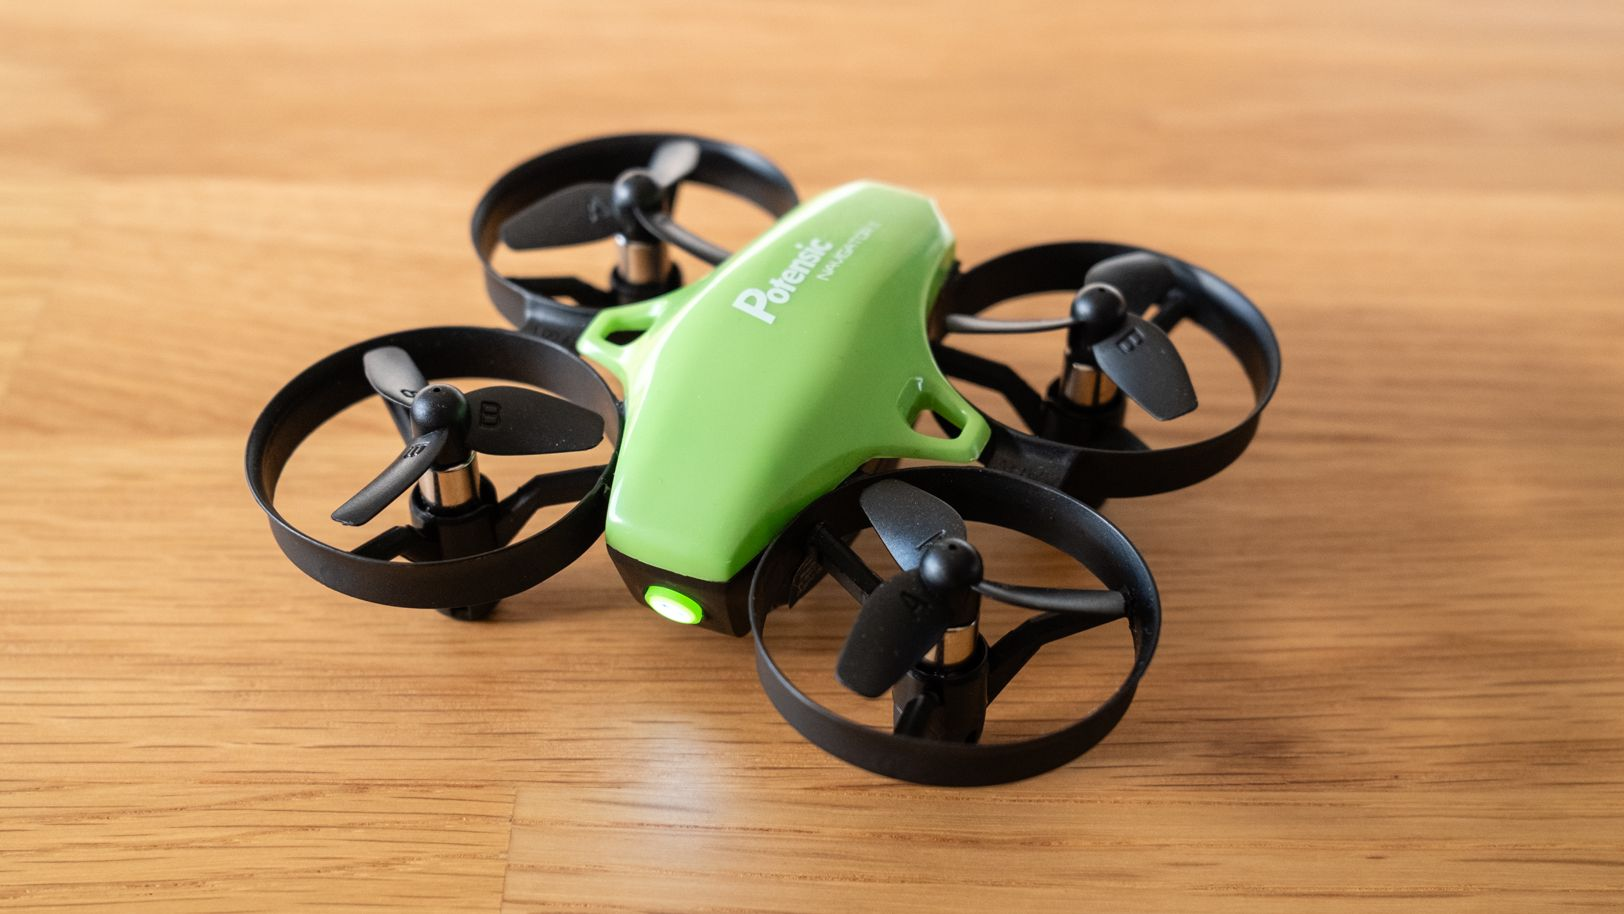
\includegraphics[width=0.4\textwidth]{img/mini-drone.JPG}
    \caption{Miniature Drone \cite{abbott2024}}
\end{figure}

The \gls{uwaal} has commissioned the development of an autonomous indoor drone capable of stable flight within confined environments. The system will be used to survey and inspect indoor areas such as garages and laboratories, following predefined flight paths while maintaining altitude and position despite external airflow disturbances. It must integrate sensing, control, communication, and power management within a compact and lightweight platform, designed from first principles to ensure safety, efficiency, and reliability. This project explores the design and implementation of such a platform, aligning with \gls{uwaal}’s objective to develop a safe, functional, and adaptable indoor drone for future research and educational applications. 

\subsection{Scope of This Report}

This report outlines the process undertaken to design and implement a functional indoor \gls{uav} for operation within confined environments. It defines the technical, safety, and regulatory boundaries within which the project was executed, as well as the methods used to evaluate performance against client-approved requirements. The scope covers system-level design, hardware and firmware integration, testing, and validation to ensure stable flight, effective altitude control, reliable communication, and essential safety functionality. 

The document also presents the rationale behind key design choices and the underlying system architecture. It details specific design aspects, including component selection, \gls{pcb} schematic design and layout, flight control algorithms, and safety mechanisms, while addressing relevant standards for electrical safety, risk management, and compliance. Consideration is given to manufacturability, maintainability, and adherence to cost and resource constraints. Beyond immediate development outcomes, the report establishes a framework that supports future extensions of the platform within the \gls{uwaal}. 

\subsection{Purpose of the Design}

The primary objective of this project is to design, develop, and validate a low-cost indoor drone capable of achieving stable flight and hovering performance without GPS-based navigation. The system is intended for use within the \gls{uwaal} to perform autonomous operations while maintaining a specified altitude and compensating for environmental disturbances such as localised airflow. 

\begin{figure}[H]
    \centering
    \captionsetup{justification=centering, margin=1cm}
    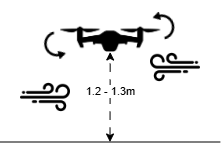
\includegraphics[width=0.4\textwidth]{img/intro-drone-gray5.PNG}
    \caption{Surveillance Drone Diagram}
\end{figure}

The proposed system architecture features a custom-designed \gls{pcb} flight controller integrating onboard power distribution, sensing, and control modules. Flight stabilisation and altitude control are achieved through sensor fusion of inertial and distance measurements processed via onboard control algorithms. The design incorporates safety features such as shrouded propellers or propeller guards, low-battery auto-landing capability, and a failsafe mechanism that triggers a controlled landing or motor shutdown following a communication loss exceeding thirty seconds. The drone operates on 1S or 2S lithium-polymer batteries with a maximum capacity of 800~mAh and must sustain a minimum flight duration of three minutes. All components and materials conform to the allocated project budget of AUD~\$350. The overarching goal is to deliver a robust, safe, and open-source indoor drone platform that satisfies all operational, safety, and budgetary requirements. 

\subsection{Background}

\glspl{uav} combine sensing, computation, and actuation to achieve controlled flight through coordinated motor thrust. Their operation depends on precise feedback control systems that maintain stability and orientation while responding to pilot or autonomous commands. This is typically accomplished using onboard microcontrollers running real-time control algorithms that process data from inertial and range sensors to dynamically adjust motor outputs.

\begin{figure}[H]
    \centering
    \captionsetup{justification=centering, margin=1cm}
    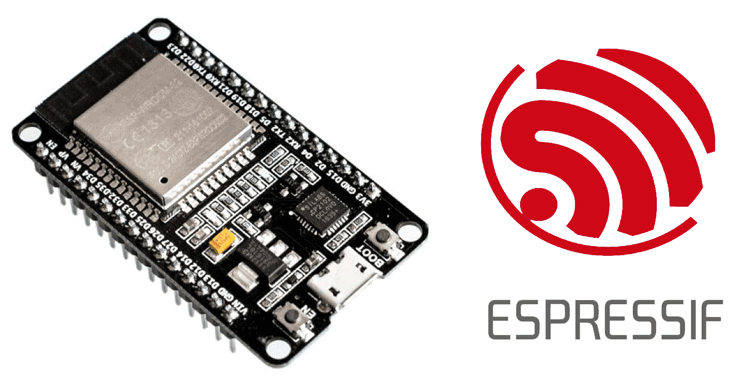
\includegraphics[width=0.42\textwidth]{img/intro-espressif.PNG}
    \caption{Espressif ESP32 DevKit~\cite{iotdesignpro2019}}
\end{figure}

\pagebreak

The ESP32 microcontroller has emerged as a compact and cost-effective solution for such systems, integrating dual-core processing, Wi-Fi connectivity, and sufficient computational power to manage both flight control and communication tasks. Its compatibility with open-source frameworks such as Espressif’s \gls{esp-idf} enables flexible low-level implementation of control loops, sensor fusion, and telemetry within a single embedded platform.

In parallel, advances in printed circuit board (\gls{pcb}) design allow integration of flight electronics, power management, and motor drivers onto lightweight, custom boards that minimise wiring and improve reliability. 

\begin{figure}[H]
    \centering
    \captionsetup{justification=centering, margin=1cm}
    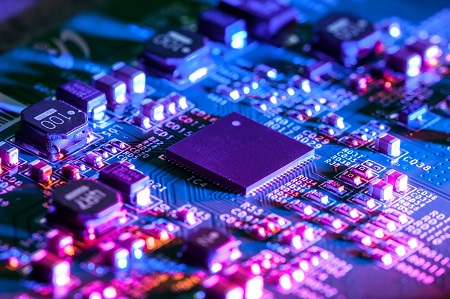
\includegraphics[width=0.4\textwidth]{img/intro-pcb.PNG}
    \caption{Printed Circuit Board \cite{mistral2020}}
\end{figure}

Together, these developments enable the creation of small-scale, low-cost autonomous drones capable of stable flight and sensor-based navigation for educational, research, and experimental applications.

\subsection{Summary of Contributions}

\begin{table}[H]
\centering
\caption{Team Member Contribution Breakdown}
\renewcommand{\arraystretch}{1.2}
\begin{tabular}{@{}lcc@{}}
\toprule
\textbf{Task} & \textbf{Sofia Khokhlenok (\%)} & \textbf{Sunny Guo (\%)} \\ 
\midrule
Conception & 50 & 50 \\
Research & 60 & 40 \\
Requirement Development & 50 & 50 \\
System Design & 70 & 30 \\
System Architecture & 50 & 50 \\
Hardware Development & 20 & 80 \\
Firmware Development & 90 & 10 \\
PCB Research & 40 & 60 \\
PCB/Frame Prototyping & 20 & 80 \\
Purchasing Electronic Materials & 50 & 50 \\
Frame Design & 15 & 85 \\
Software Debugging and Testing & 80 & 20 \\
Hardware Debugging and Testing & 20 & 80 \\
Overall Prototype Testing & 50 & 50 \\
Management and Organization & 80 & 20 \\
Final Report & 55 & 45 \\
\textbf{Average} & 50 & 50 \\
\bottomrule
\end{tabular}
\end{table}

\subsection{Report Structure}
This report provides a comprehensive overview of the design, development, and evaluation of the autonomous ESP32-based indoor surveillance drone. 

\textbf{Section~1} introduces the project, outlining its scope, purpose, background, and summary of contributions. It also describes the overall report structure to guide the reader. 

\textbf{Section~2} presents the detailed design process, including system requirements, overall and subsystem architecture (hardware, firmware, and justification), and individual design elements such as PCB components, frame design, and firmware modules. It further describes testing procedures—covering hardware verification, stationary and dynamic testing—as well as system integration, stakeholder engagement, safety, ethical considerations, and risk analysis. The section concludes with assembly procedures, design outputs, and final cost breakdowns.

\textbf{Section~3} outlines recommendations for future improvements and potential extensions of the system. 

\textbf{Section~4} serves as a user manual, providing detailed instructions for operation, maintenance, and troubleshooting. 

\textbf{Section~5} lists all referenced materials and supporting documentation. 

Finally, \textbf{the Appendices} contain supplementary materials, including design constraints, requirements updates, prototype details, additional figures, and complete firmware source code listings.
